\section{پیوست}\label{sec:appendix}
در این بخش نمودارهای الگوریتم \lr{PSO}
آورده شده است.
 \begin{figure}[H]
	\caption{نمودار همگرایی الگوریتم \lr{PSO} تابع شماره یک ($D=10$) برای ۱۰۰۰ تکرار } 
	\centering 
	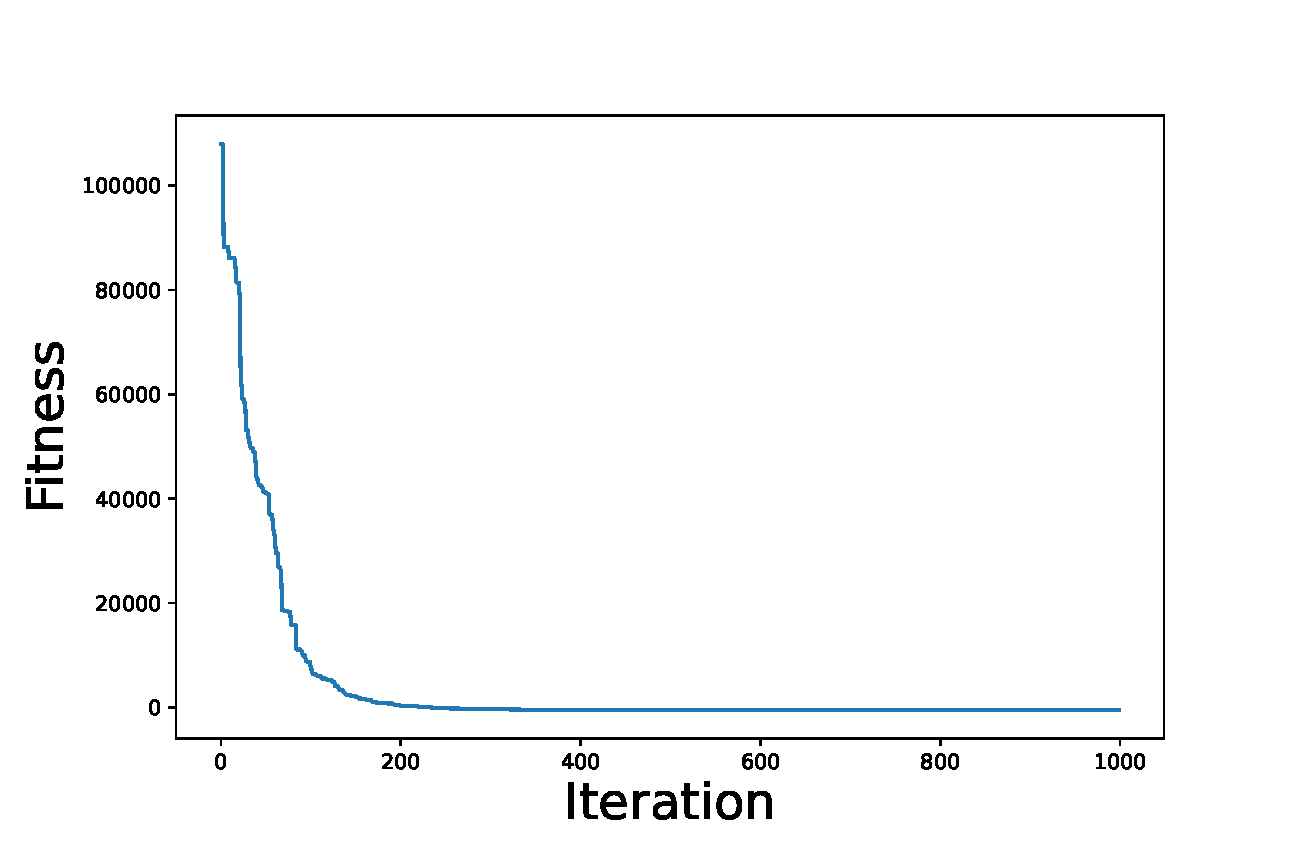
\includegraphics[width=16cm]{../Figure/Q1/PSO_convergence_curve_10_ite_1000} 
\end{figure}

 \begin{figure}[H]
	\caption{نمودار همگرایی الگوریتم \lr{PSO} تابع شماره یک ($D=10$) برای ۱۰۰۰۰ تکرار } 
	\centering 
	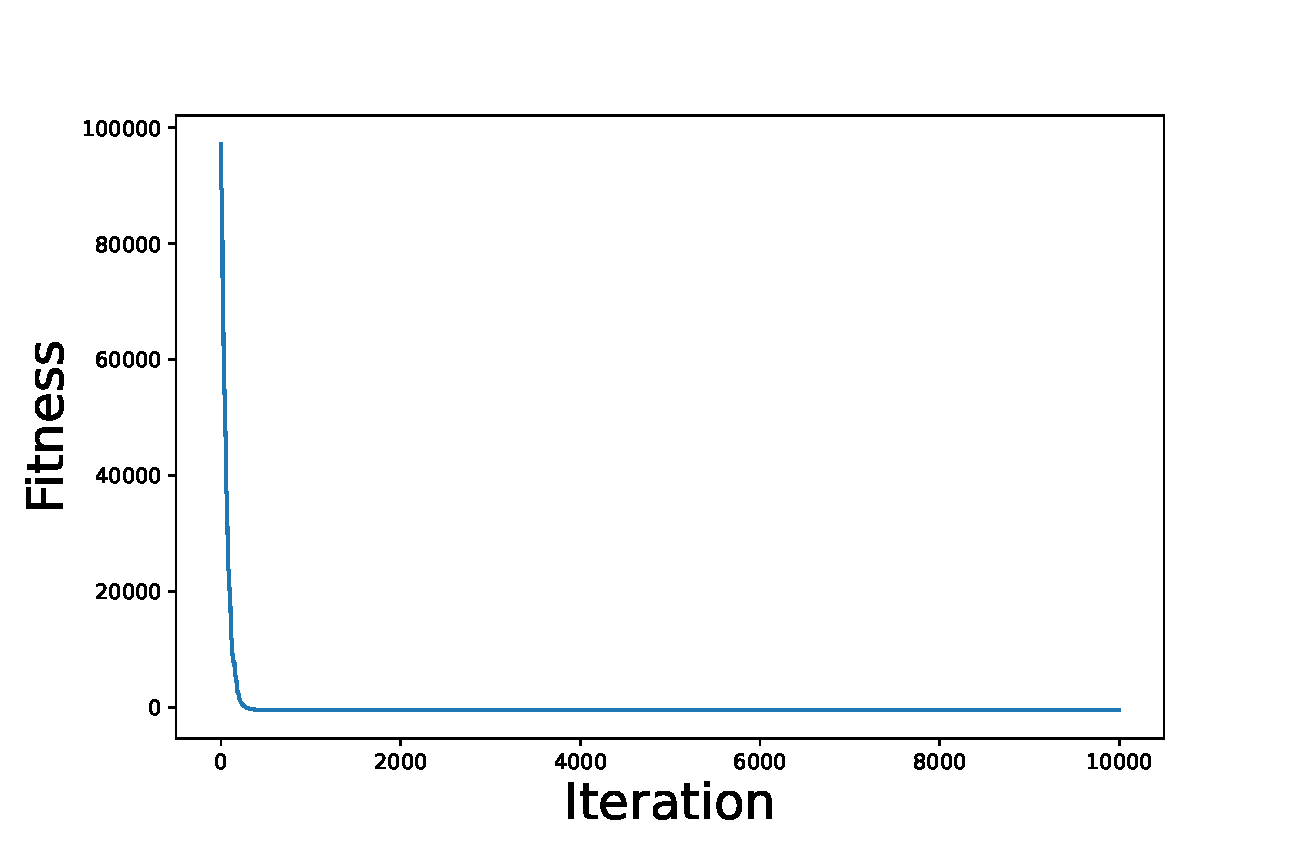
\includegraphics[width=16cm]{../Figure/Q1/PSO_convergence_curve_10_ite_10000} 
\end{figure}

 \begin{figure}[H]
	\caption{نمودار همگرایی الگوریتم \lr{PSO} تابع شماره یک ($D=10$) برای ۱۰۰۰۰۰ تکرار } 
	\centering 
	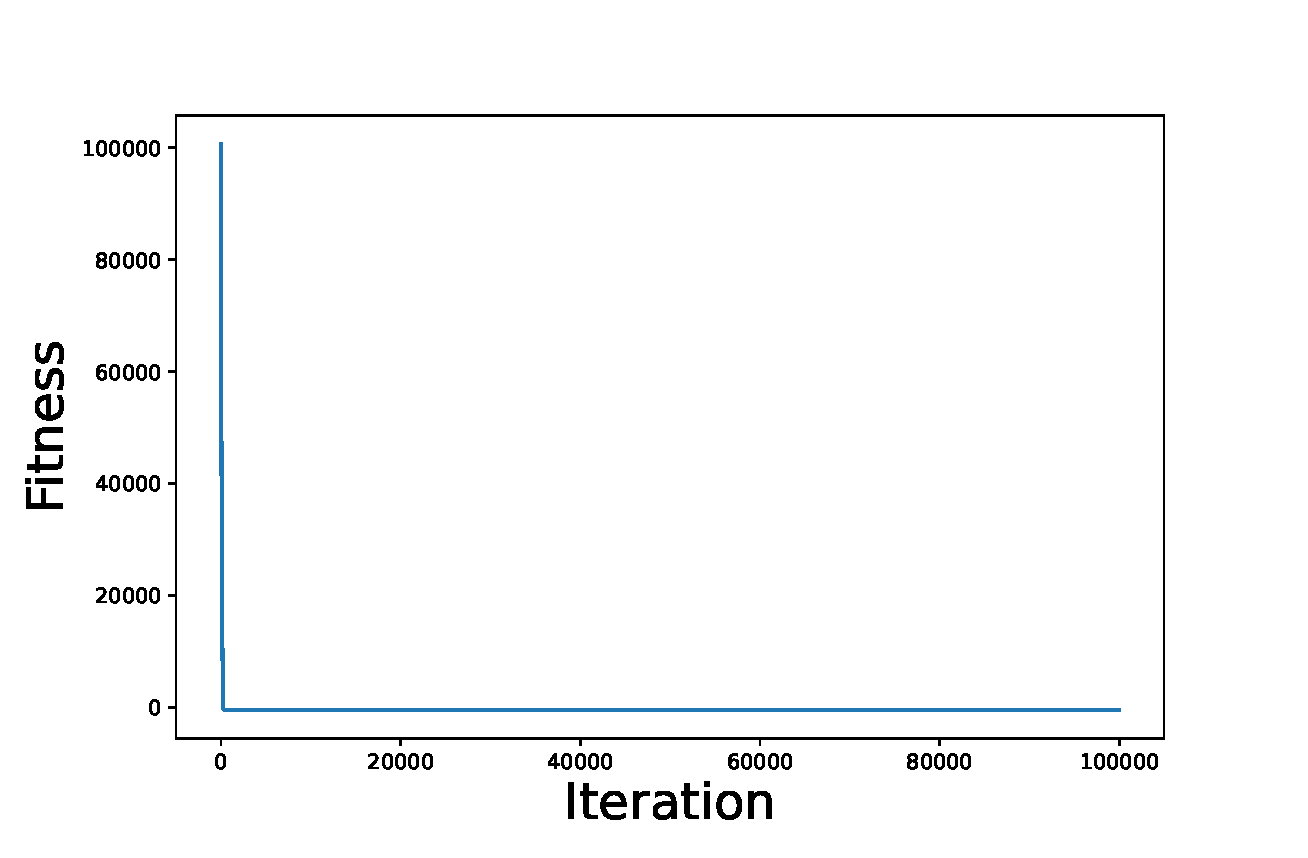
\includegraphics[width=16cm]{../Figure/Q1/PSO_convergence_curve_10_ite_100000} 
\end{figure}



 \begin{figure}[H]
	\caption{نمودار همگرایی الگوریتم \lr{PSO} تابع شماره یک ($D=30$) برای ۱۰۰۰ تکرار } 
	\centering 
	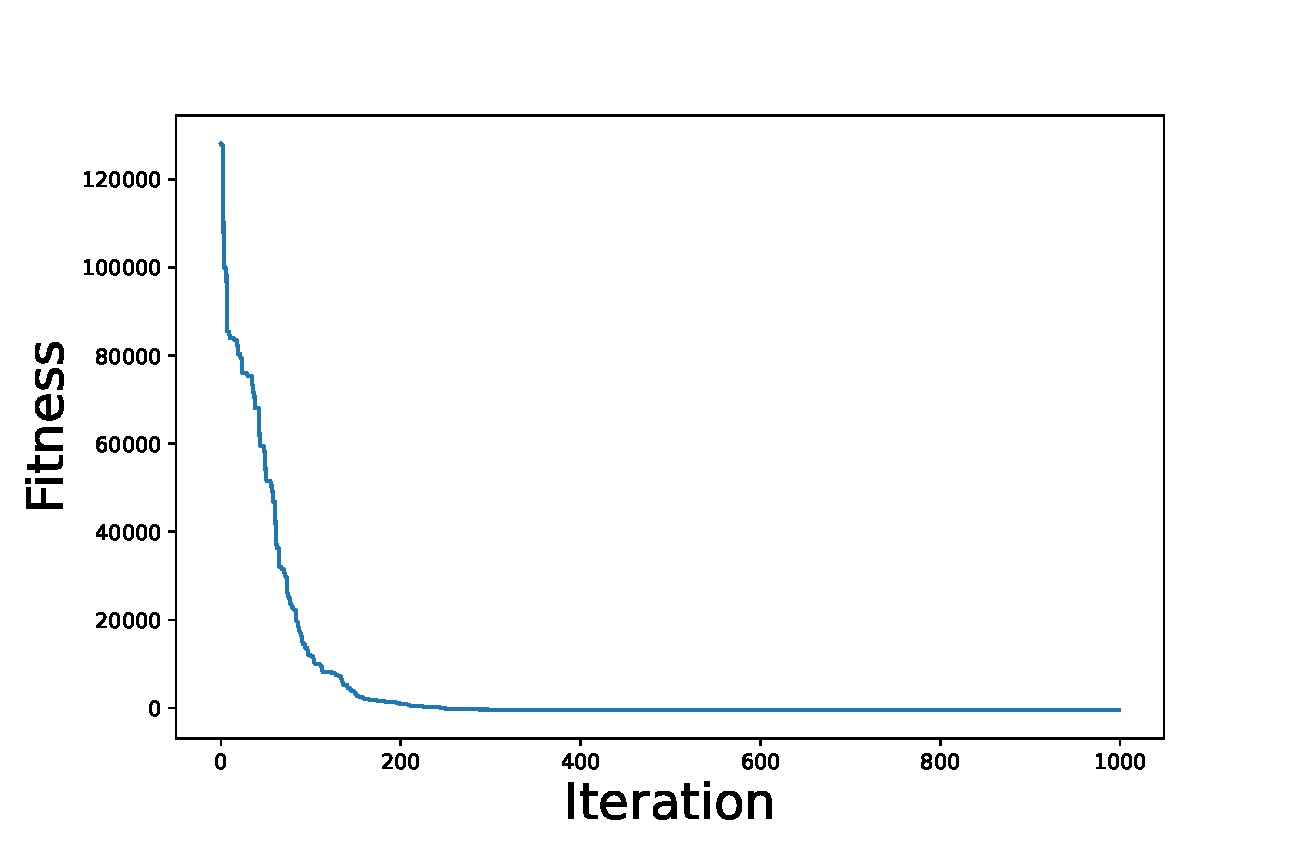
\includegraphics[width=16cm]{../Figure/Q1/PSO_convergence_curve_30_ite_1000} 
\end{figure}

\begin{figure}[H]
	\caption{نمودار همگرایی الگوریتم \lr{PSO} تابع شماره یک ($D=30$) برای ۱۰۰۰۰ تکرار } 
	\centering 
	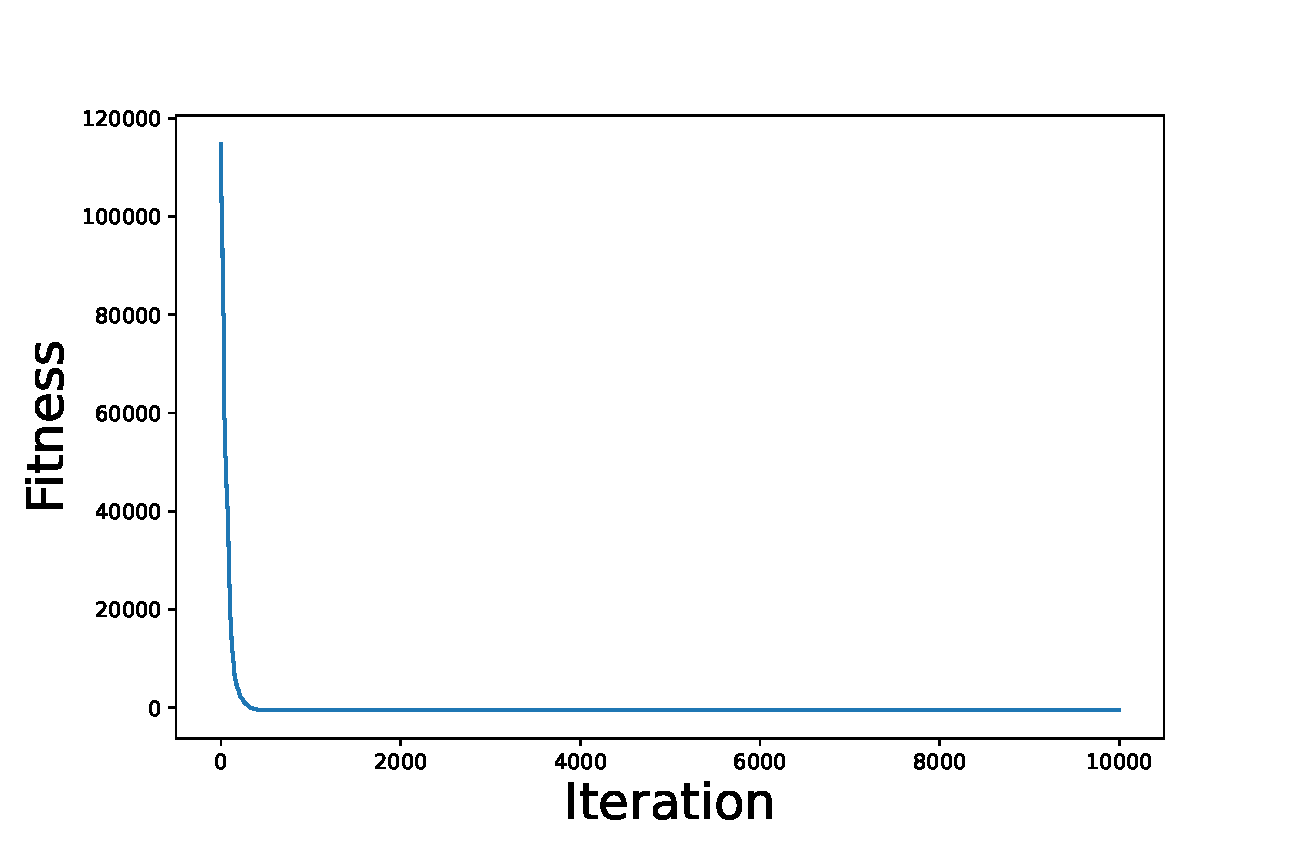
\includegraphics[width=16cm]{../Figure/Q1/PSO_convergence_curve_30_ite_10000} 
\end{figure}

\begin{figure}[H]
	\caption{نمودار همگرایی الگوریتم \lr{PSO} تابع شماره یک ($D=30$) برای ۱۰۰۰۰۰ تکرار } 
	\centering 
	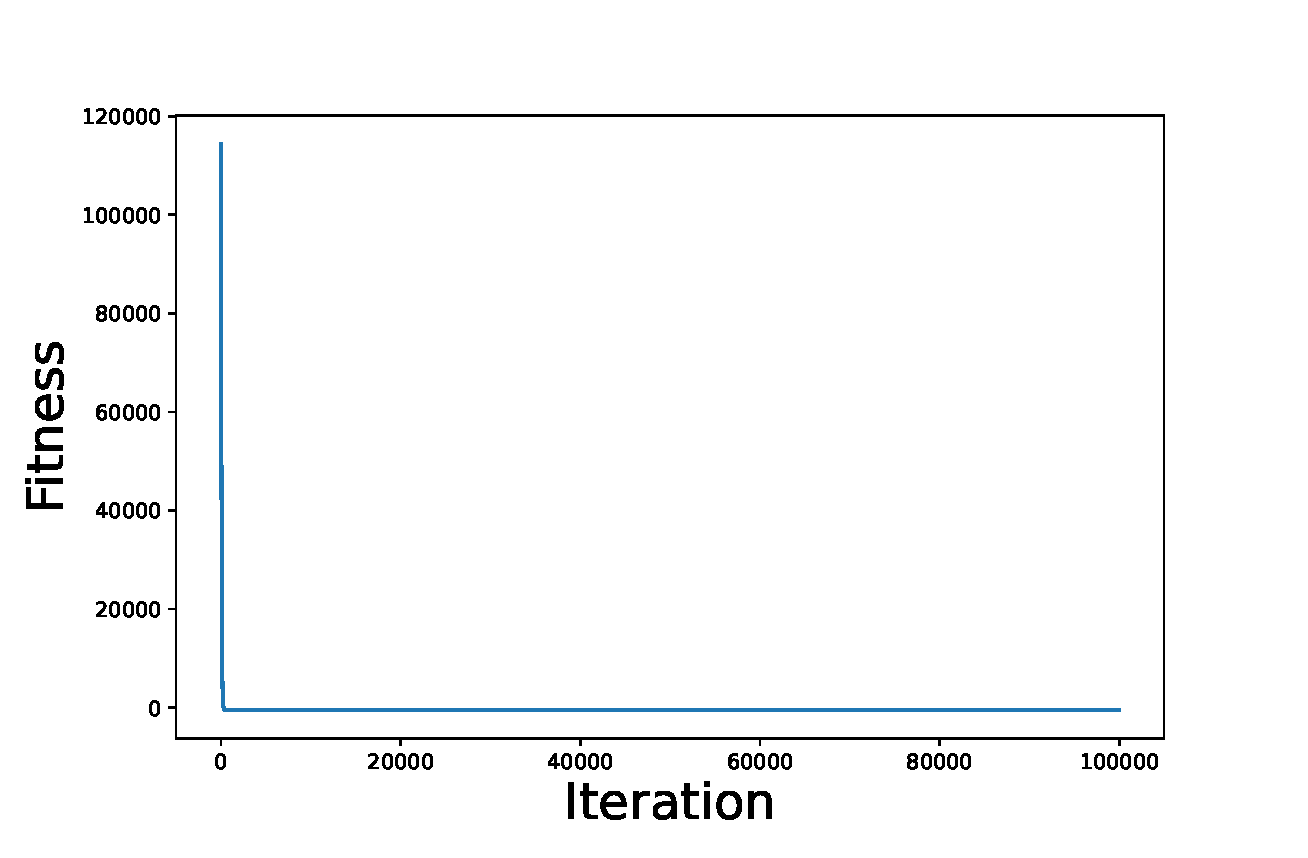
\includegraphics[width=16cm]{../Figure/Q1/PSO_convergence_curve_30_ite_100000} 
\end{figure}


 \begin{figure}[H]
	\caption{نمودار همگرایی الگوریتم \lr{PSO} تابع شماره یک ($D=50$) برای ۱۰۰۰ تکرار } 
	\centering 
	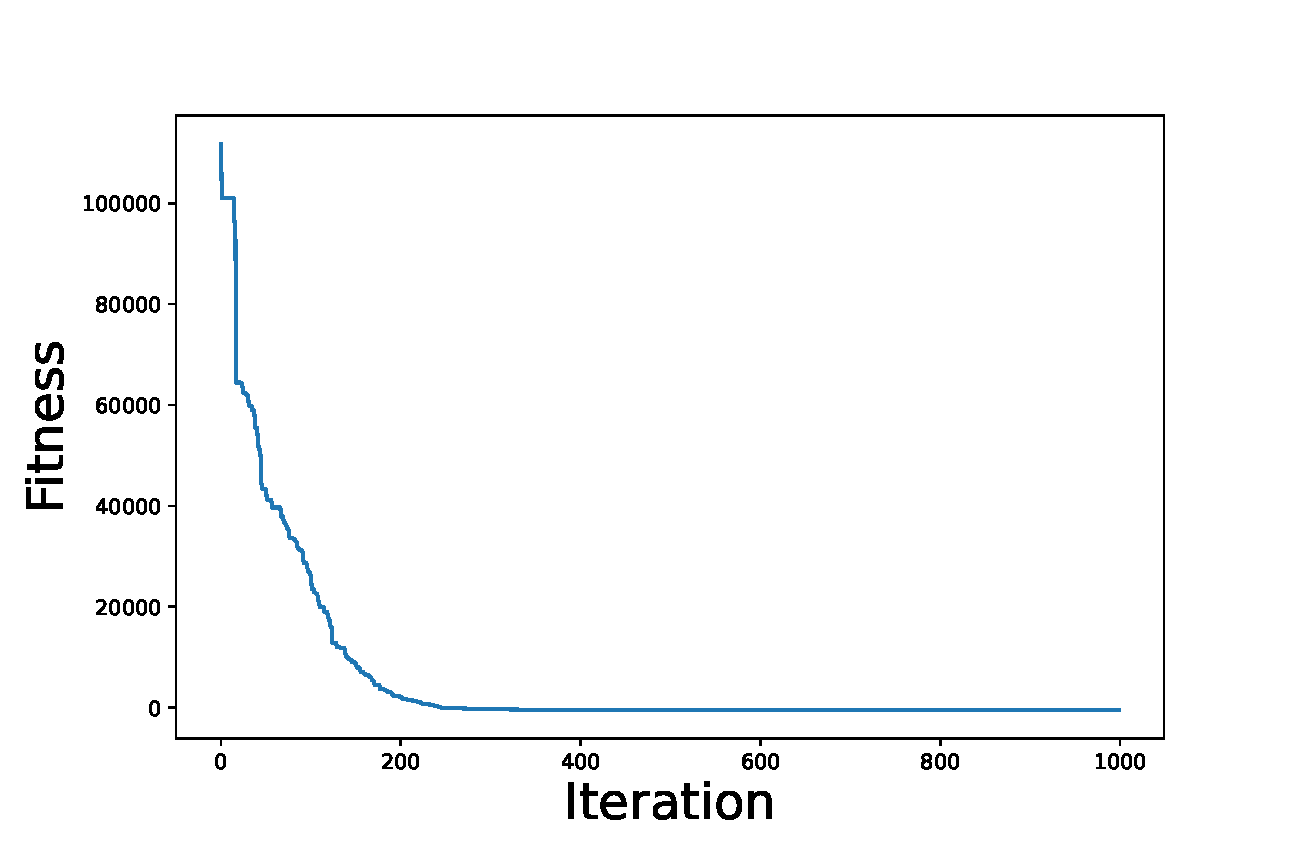
\includegraphics[width=16cm]{../Figure/Q1/PSO_convergence_curve_50_ite_1000} 
\end{figure}

\begin{figure}[H]
	\caption{نمودار همگرایی الگوریتم \lr{PSO} تابع شماره یک ($D=50$) برای ۱۰۰۰۰ تکرار } 
	\centering 
	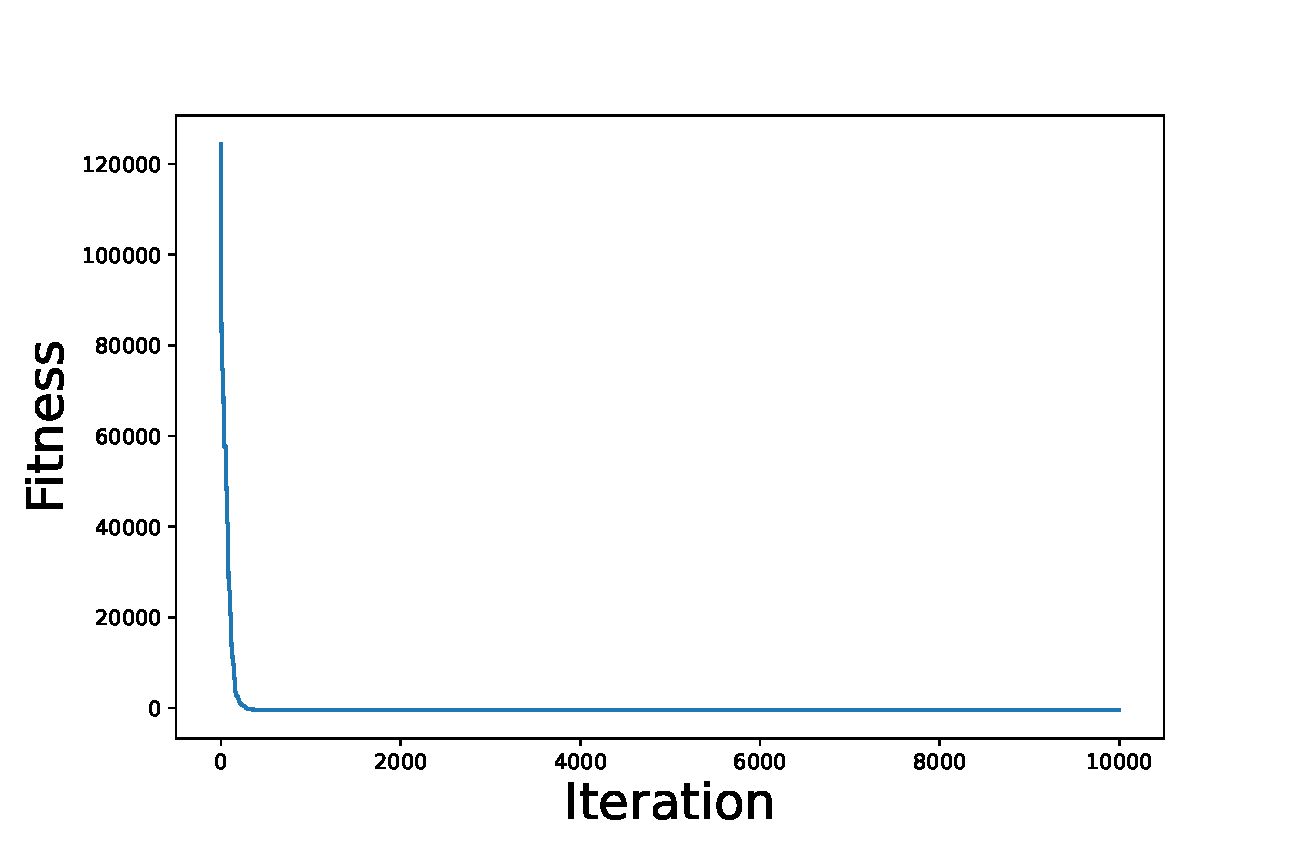
\includegraphics[width=16cm]{../Figure/Q1/PSO_convergence_curve_50_ite_10000} 
\end{figure}

\begin{figure}[H]
	\caption{نمودار همگرایی الگوریتم \lr{PSO} تابع شماره یک ($D=50$) برای ۱۰۰۰۰۰ تکرار } 
	\centering 
	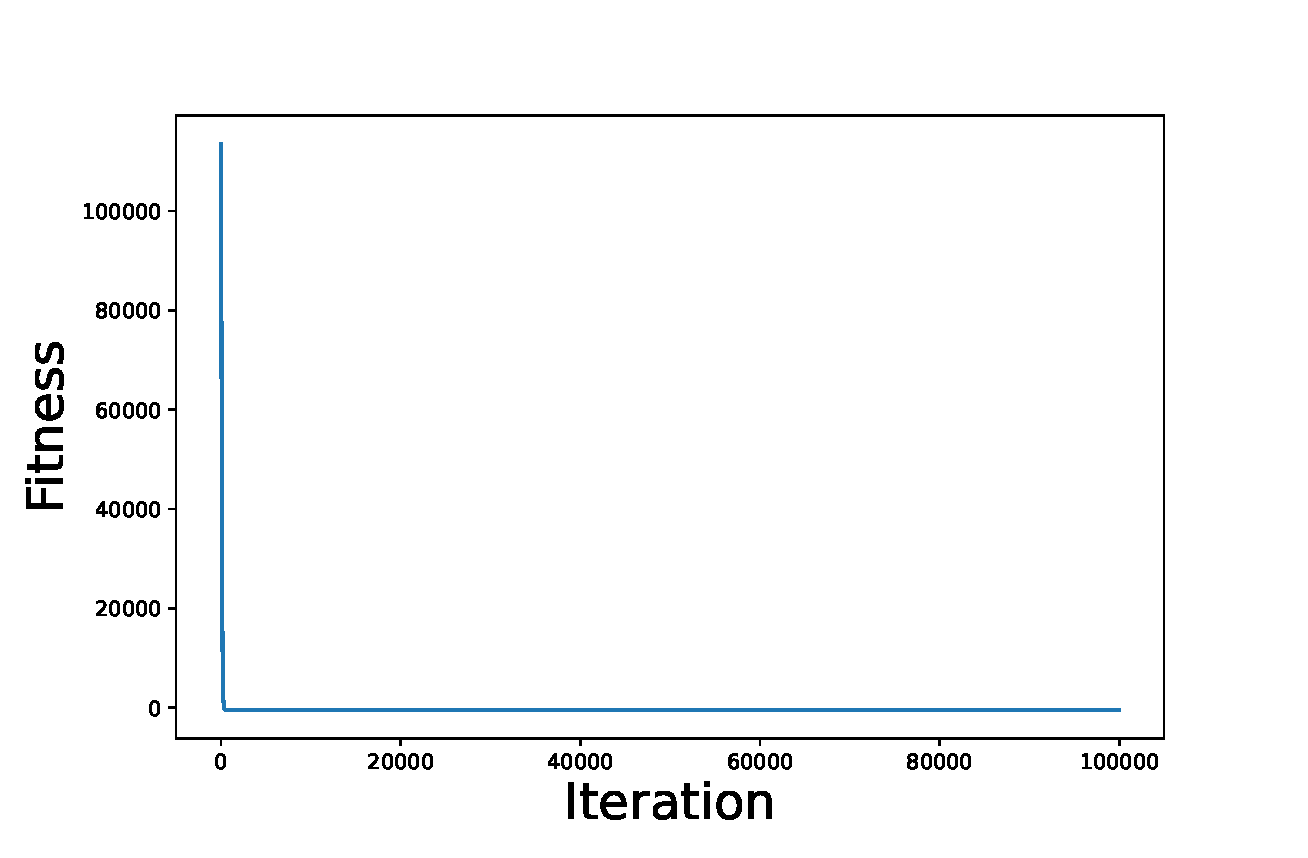
\includegraphics[width=16cm]{../Figure/Q1/PSO_convergence_curve_50_ite_100000} 
\end{figure}




 \begin{figure}[H]
	\caption{نمودار همگرایی الگوریتم \lr{PSO} تابع شماره دو ($D=10$) برای ۱۰۰۰ تکرار } 
	\centering 
	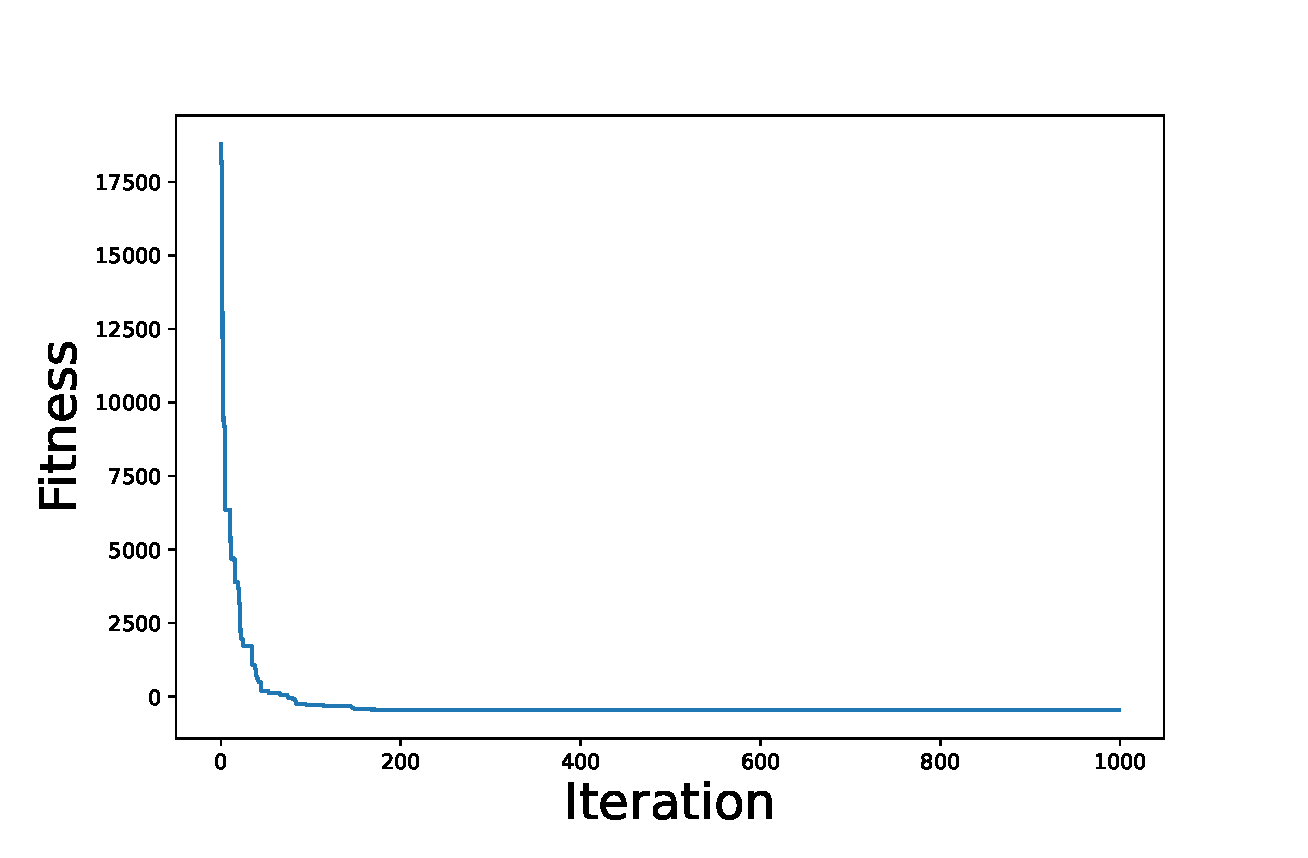
\includegraphics[width=16cm]{../Figure/Q1/PSO_II_convergence_curve_10_ite_1000} 
\end{figure}


\begin{figure}[H]
	\caption{نمودار همگرایی الگوریتم \lr{PSO} تابع شماره دو ($D=10$) برای ۱۰۰۰۰۰ تکرار } 
	\centering 
	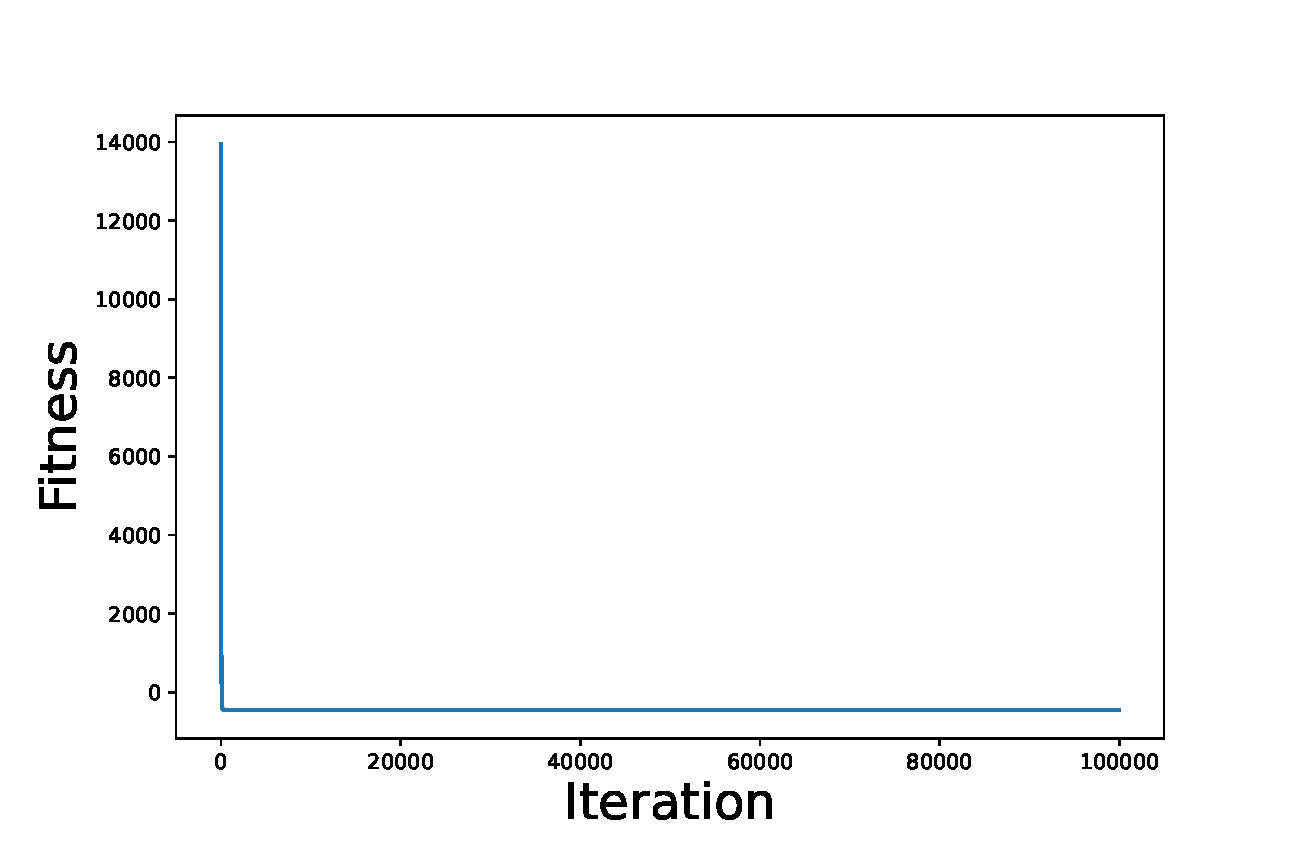
\includegraphics[width=16cm]{../Figure/Q1/PSO_II_convergence_curve_10_ite_100000} 
\end{figure}

 \begin{figure}[H]
	\caption{نمودار همگرایی الگوریتم \lr{PSO} تابع شماره دو ($D=30$) برای ۱۰۰۰ تکرار } 
	\centering 
	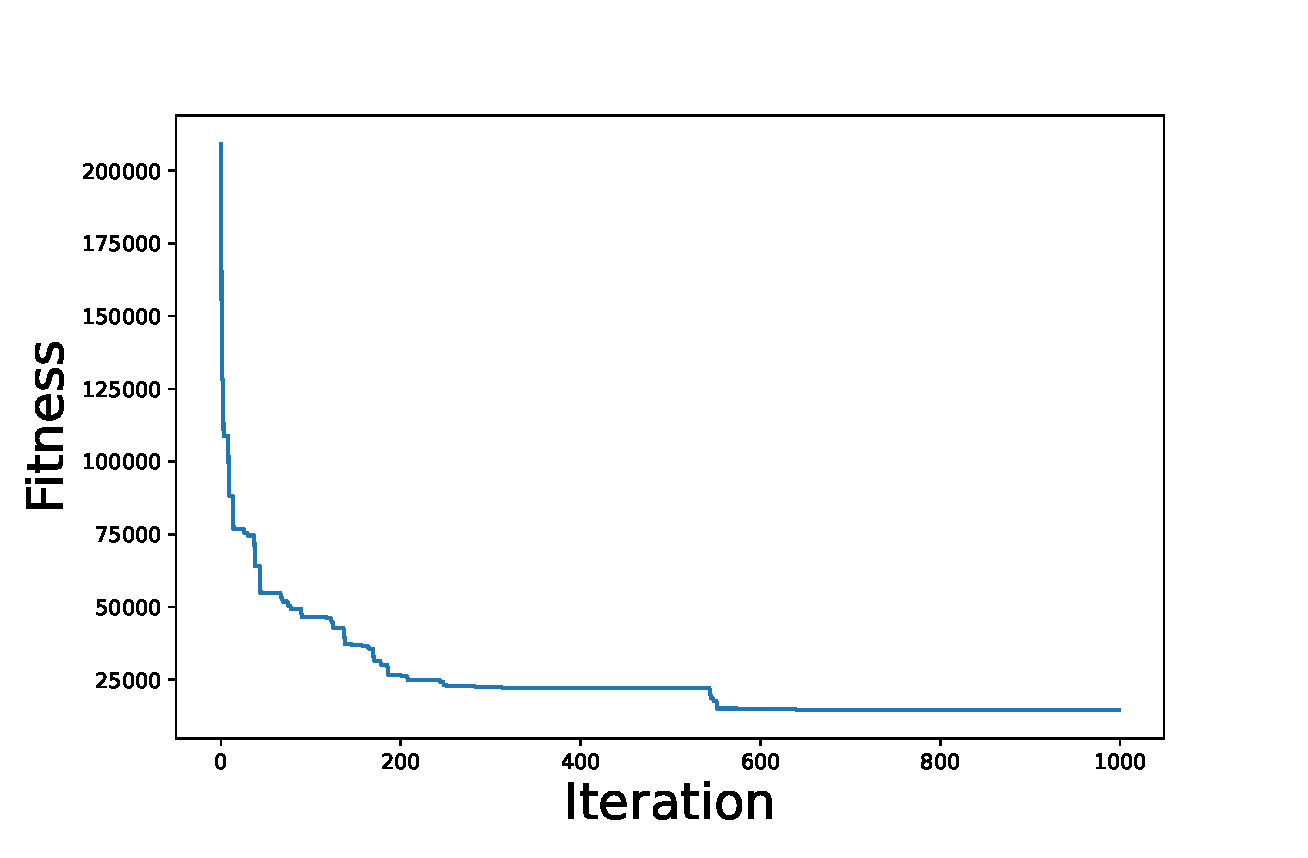
\includegraphics[width=16cm]{../Figure/Q1/PSO_II_convergence_curve_30_ite_1000} 
\end{figure}

 \begin{figure}[H]
	\caption{نمودار همگرایی الگوریتم \lr{PSO} تابع شماره دو ($D=30$) برای ۱۰۰۰۰۰ تکرار } 
	\centering 
	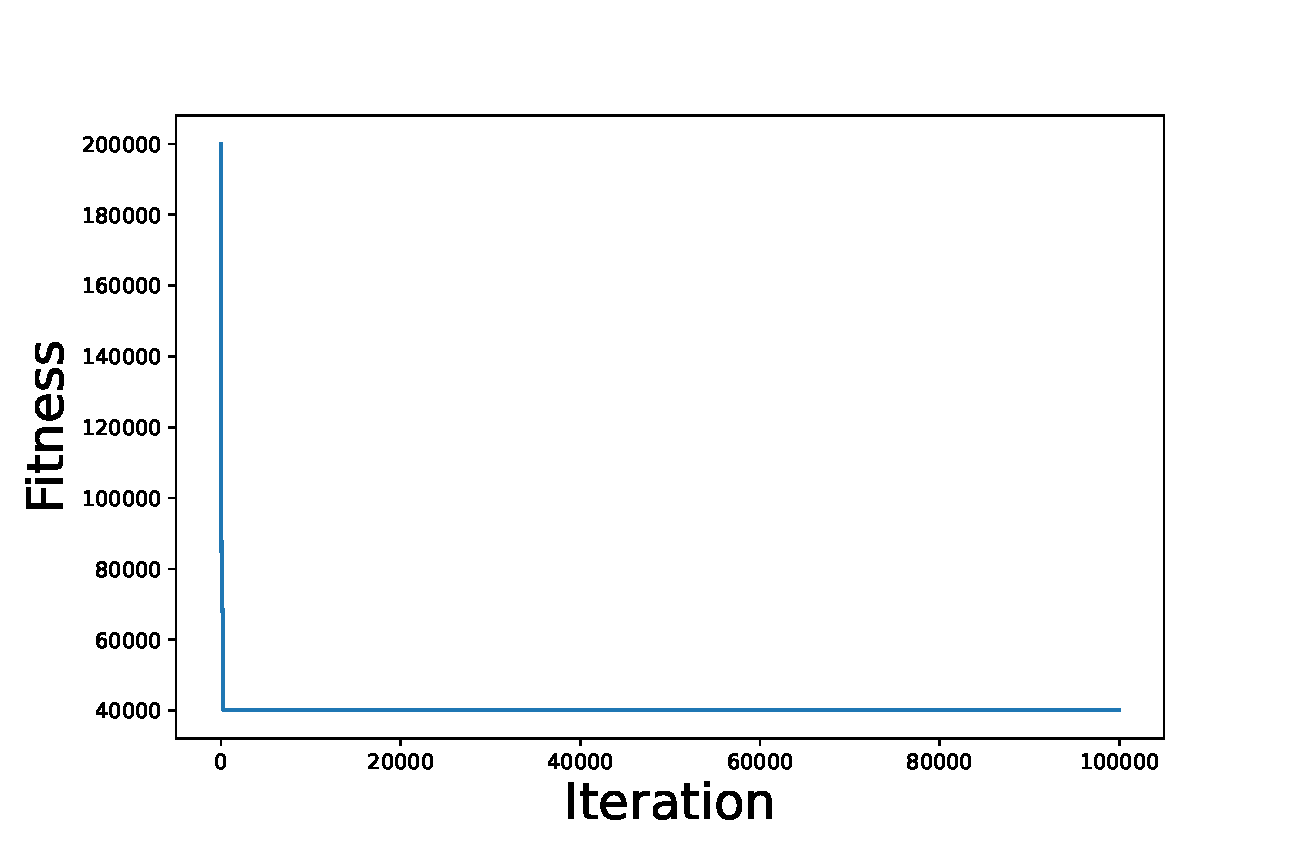
\includegraphics[width=16cm]{../Figure/Q1/PSO_II_convergence_curve_30_ite_100000} 
\end{figure}

 \begin{figure}[H]
	\caption{نمودار همگرایی الگوریتم \lr{PSO} تابع شماره دو ($D=50$) برای ۱۰۰۰ تکرار } 
	\centering 
	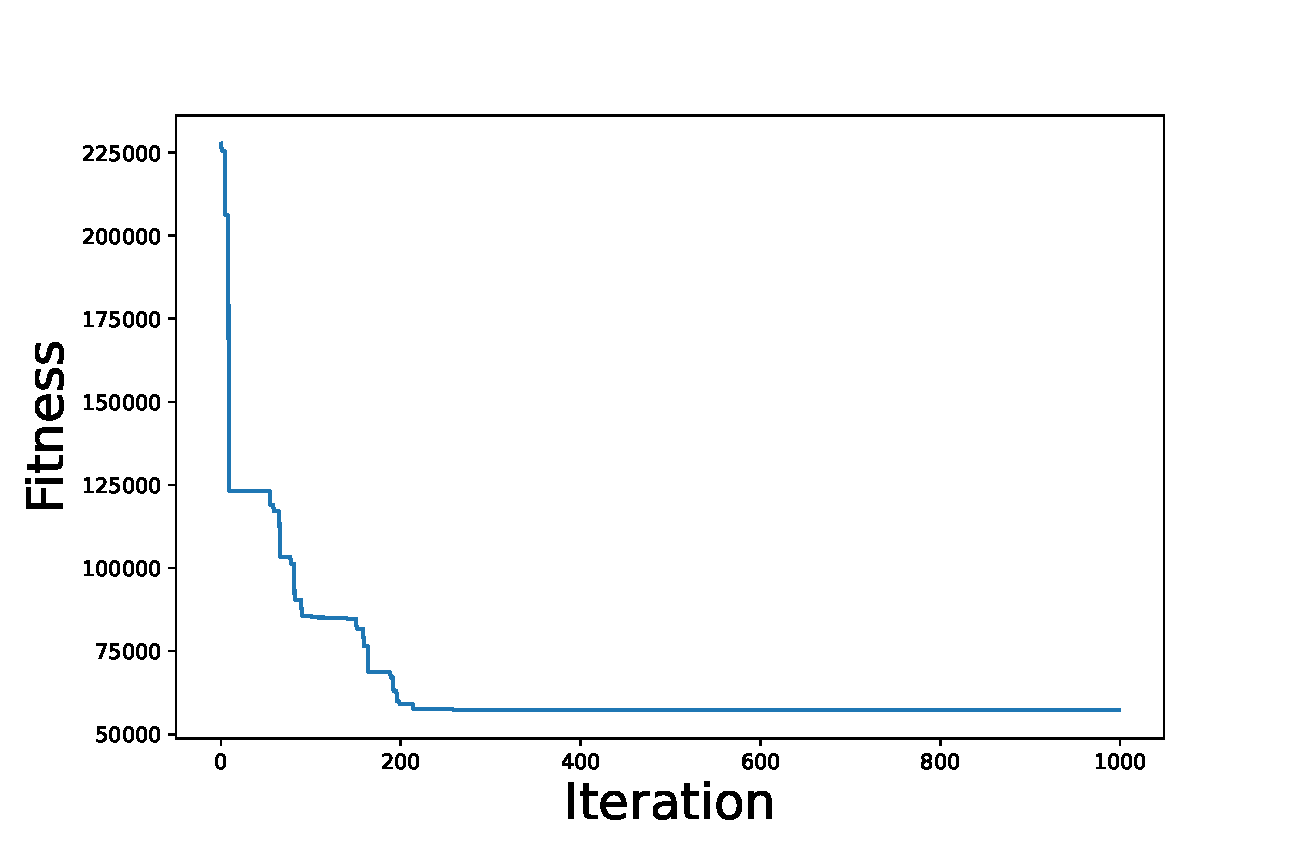
\includegraphics[width=16cm]{../Figure/Q1/PSO_II_convergence_curve_50_ite_1000} 
\end{figure}


